\section{Methods}

\subsection{Notation}

In the following, we will use definitions and notations introduced by \citep{rougier:2011} where a neural map is defined as the projection from a manifold $\Omega \subset \mathbb{R}^d$ onto a set $\mathcal{N}$ of $n$ {\em  neuron}s which is formally written as $\Phi : \Omega \rightarrow \mathcal{N}$. Each neuron $i$ is associated with a code word $\mathbf{w}_i \in \mathbb{R}^d$, all of which establish the set  $\{\mathbf{w}_i\}_{i \in   \mathcal{N}}$ that is referred as the code book. The mapping from $\Omega$ to $\mathcal{N}$ is a closest-neighbor winner-take-all rule such that any vector $\mathbf{v} \in \Omega$ is mapped to a neuron $i$ with the code $\mathbf{w}_\mathbf{v}$ being closest to the actual presented stimulus vector $\mathbf{v}$,
\begin{equation}
\Phi : \mathbf{v} \mapsto argmin_{i \in \mathcal{N}} (\lVert \mathbf{v} -
\mathbf{w}_i \rVert).
\label{eq:psi}
\end{equation}
The neuron $\mathbf{w}_\mathbf{v}$ is named the best matching unit (BMU) and the set $C_i = \{x \in \Omega | \Phi(x) = \mathbf{w}_i \}$ defines the {\em receptive field} of the neuron $i$.


%Before we present our new SOM learning algorithm, we introduce the notation  and terminology we are using throughout the present work. We borrow the notation from a previous work \citep{rougier:2011}.  A neural map is defined to be the projection from a manifold $\Omega \subset \mathbb{R}^d$ onto a set $\mathcal{N}$ of $n$ {\em neuron}s $\Phi : \Omega \rightarrow \mathcal{N}$. Each neuron $i$ is associated with a code word $\mathbf{w}_i \in \mathbb{R}^d$, all of which establish the set  $\mathcal{W} = \{\mathbf{w}_i, i \in \mathcal{N}\}$ that is referred as the code book. The mapping from $\Omega$ to $\mathcal{N}$ is a closest-neighbor winner-take-all rule such that any vector $\mathbf{v} \in \Omega$ is mapped to a neuron $i$ with the code $\mathbf{w}_\mathbf{v}$ being closest to the current input vector $\mathbf{v}$,
%\begin{equation}
%\Phi : \mathbf{v} \mapsto argmin_{i \in \mathcal{N}} (\lVert \mathbf{v} -
%\mathbf{w}_i \rVert).
%\label{eq:psi}
%\end{equation}
%The neuron $\mathbf{w}_\mathbf{v}$ is named the best matching unit (BMU) and the set $C_i = \{x \in \Omega | \Phi(x) = \mathbf{w}_i \}$ defines the {\em receptive field} of neuron $i$.


\subsection{Spatial distribution} % \& Centroidal Voronoi Tesselation}
\label{sec:spatial_dist}

The SOM space is usually defined as a two-dimensional region where nodes are arranged in a regular lattice (rectangular or hexagonal). Here, we consider instead the random placement of neurons with a specific spectral distribution (blue noise). As explained in \citep{Zhou:2012}, the spectral distribution property of noise patterns is often described in terms of the Fourier spectrum color. White noise corresponds to a flat spectrum with equal energy distributed in all frequency bands while blue noise has weak low-frequency energy, but strong high-frequency energy. In other words, blue noise has intuitively good properties with points evenly spread without visible structure (see figure~\ref{fig:sampling} for a comparison of spatial distributions).
%%
\begin{figure}[htbp]
  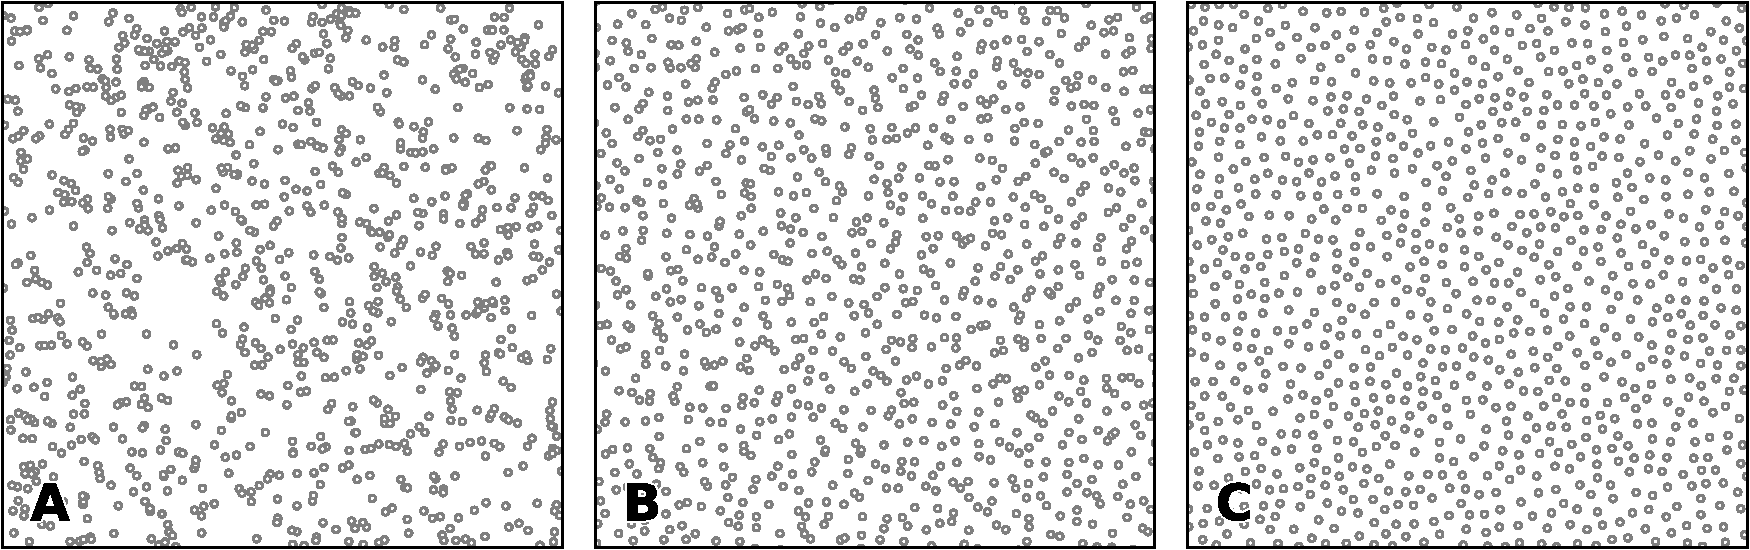
\includegraphics[width=\textwidth]{figure-blue-noise.pdf}
  \caption{\textbf{Spatial distributions.}
    \textbf{\textsf{A.}} Uniform sampling (n=1000) corresponding to white noise.
    \textbf{\textsf{B.}} Regular grid (n=32$\times$32) + jitter (2.5\%).
    \textbf{\textsf{C.}} Poisson disc sampling (n=988) corresponding to blue noise.}
  \label{fig:sampling}
\end{figure}
%%
There exists several methods \citep{Lagae:2008} to obtain blue noise sampling that have been originally designed for computer graphics (e.g. Poisson disk sampling, dart throwing, relaxation, tiling, etc.). Among these methods, the fast Poisson disk sampling in arbitrary dimensions \citep{Bridson:2007} is among the fastest ($\mathcal{O}(n)$) and easiest to use. This is the one we retained for the placement of neurons over the normalized region $[0,1]\times[0,1]$. Such Poisson disk sampling guarantees that samples are no closer to each other than a specified minimum radius. This initial placement is further refined by applying a LLoyd relaxation \citep{Lloyd:1982} scheme for 10 iterations, achieving a quasi centroidal Voronoi tesselation.


%The SOM space is usually defined as a two-dimensional manifold where nodes are arranged in a regular lattice (rectangular or hexagonal). Here, we follow a  different approach and, instead of the regular lattice, we place the neurons randomly by sampling a specific spectral distribution. More specifically, we assign neurons positions by drawing samples from a blue noise distribution. \citep{Zhou:2012}. have shown that the spectral distribution property of noise patterns is often described in terms of the Fourier spectrum color. For instance, white noise corresponds to a flat spectrum with signal's energy equally distributed to all frequency bands while blue  noise has weak low-frequency energy and strong high-frequency energy. An interesting property of the blue noise distribution is that  the resulting positions of neurons drawn are evenly spread without any apparent structure (see figure~\ref{fig:sampling} for a comparison of spatial distributions).
%%
%\begin{figure}[htbp]
%  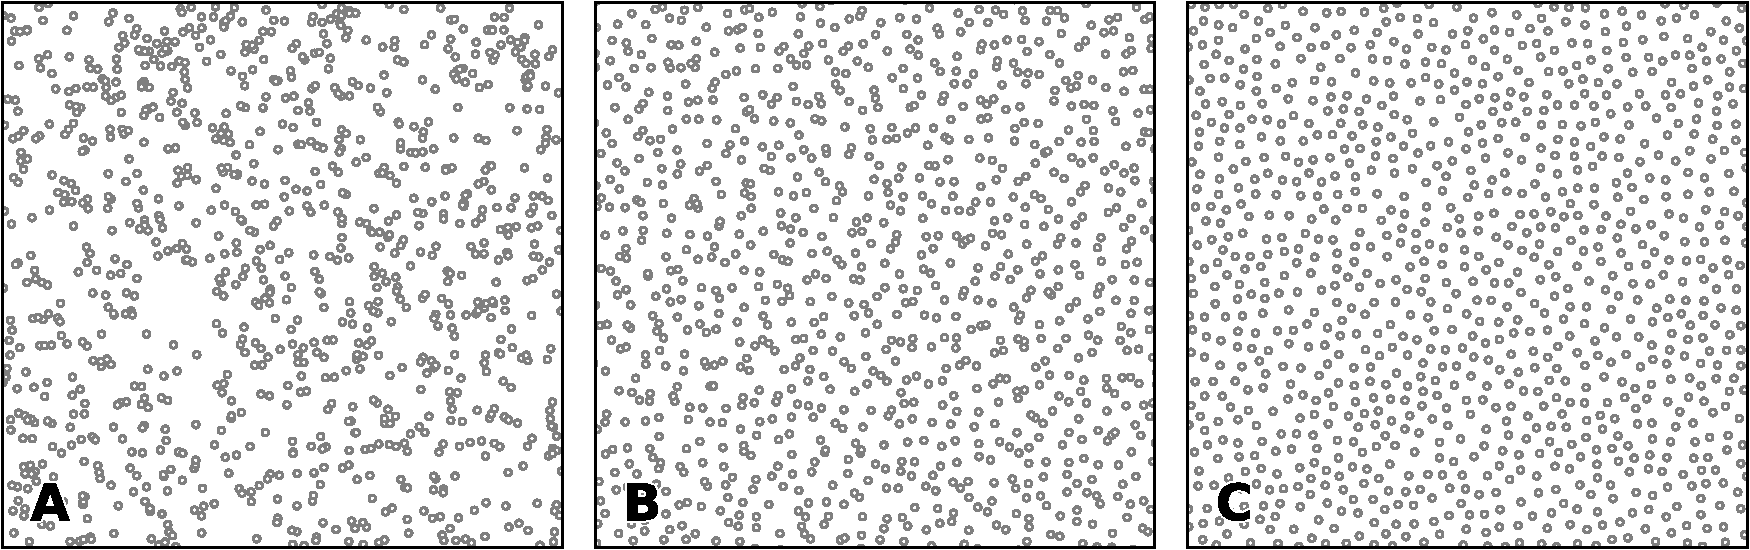
\includegraphics[width=\textwidth]{figures/blue-noise.pdf}
%  \caption{\textbf{Spatial distributions.}
%    \textbf{\textsf{A.}} Uniform sampling (n=1000) corresponding to white noise.
%    \textbf{\textsf{B.}} Regular grid (n=32$\times$32) + jitter (2.5\%).
%    \textbf{\textsf{C.}} Poisson disc sampling (n=988) corresponding to blue noise.}
%  \label{fig:sampling}
%\end{figure}
%%

%Blue noise distributions have been used in the field of computer graphics for many years and there are manych different techniques for computing them: Poisson disk sampling, dart throwing, relaxation, tiling, and other applications (see \citep{Lagae:2008} for a review). One of the fastest and easiest to implement method for generating blue noise samples is the  fast Poisson disk sampling. This method, introduced by \citep{Bridson:2007}, can be used on arbitrary dimensions in linear time ($\mathcal{O}(n)$). In this work, we propose to use this method for placing neurons over a normalized  region of $[0,1]\times[0,1]$. Such Poisson disk sampling guarantees that samples are no closer to each other than a specified minimum radius. This initial placement is further refined by applying a Lloyd relaxation~\cite{Lloyd:1982} scheme for $10$ iterations to achieve a quasi centroidal Voronoi tesselation.

\subsection{Topology}
\label{sec:topo}

Considering a set of $n$ points $P = \{P_i\}_{i \in [1,n]}$ on a finite region,
we first compute the Euclidean distance matrix $E$, where $e_{ij} = \lVert P_i - P_j \rVert$ 
and we subsequently define a connectivity matrix $G^{p}$
%= \{G^{p}_{ij}\}_{i,j \in [1,n]}$ \gid{$G^{p} = g^{p}_{ij},\, \text{where } i,j \in [1,n]$}
such that only the $p$ closest points
are connected. More precisely, if $P_j$ is among the $p$ closest neighbours of
$P_i$ then $g^p_{ij} = 1$ else we have $g^p_{ij} = 0$.
From this connectivity
matrix representing a graph, we compute the length of the shortest path between
each pair of nodes and stored them into a distance matrix $D^p$. Note that
lengths are measured in the number of nodes between two nodes such that two
nearby points (relatively to the Euclidean distance) may have a corresponding
long graph distance as illustrated in figure \ref{fig:topology}. This matrix
distance is then normalized by dividing it by the maximum distance between two
nodes such that the maximum distance in the matrix is 1. In the singular case
when two nodes cannot be connected through the graph, we recompute a spatial
distribution until all nodes can be connected.
%%
\begin{figure}
  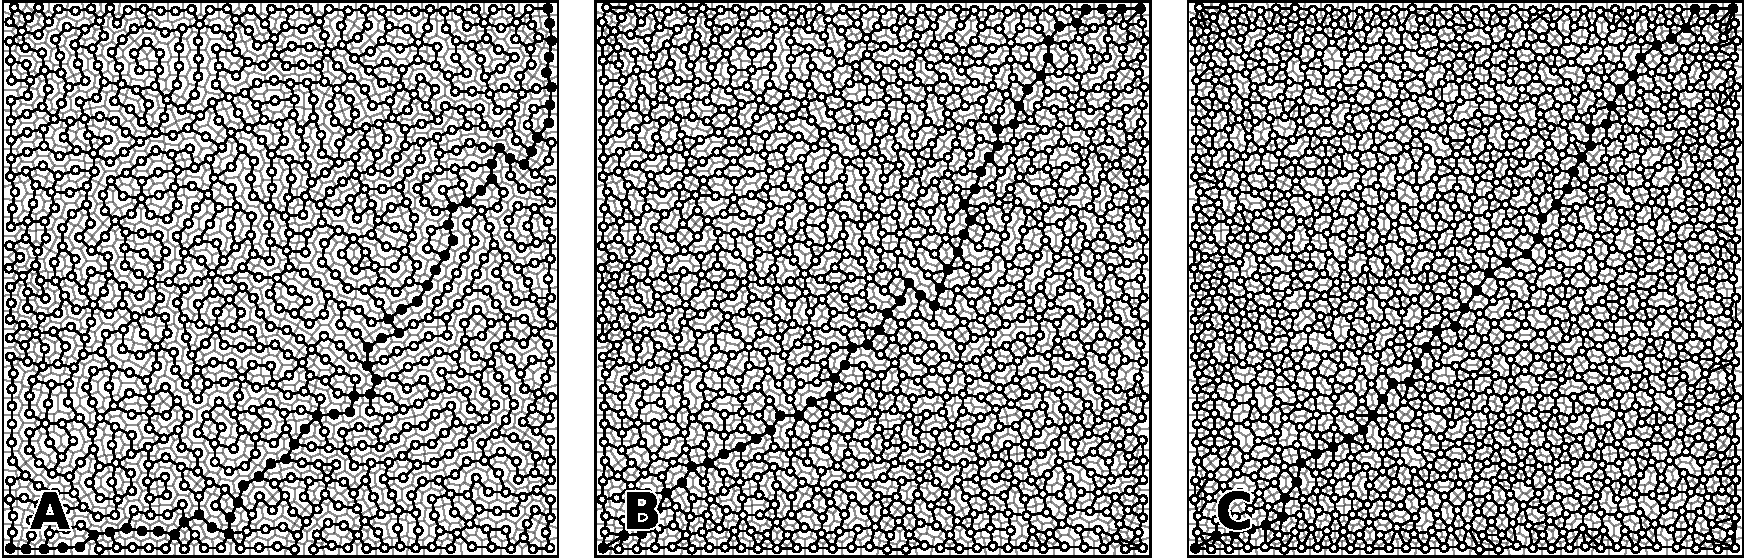
\includegraphics[width=\columnwidth]{figure-distances.pdf}
  \caption{\textbf{Influence of the number of neighbours on the graph
    distance.} The same initial set of 1003 neurons has been equiped with
    2-nearest neighbors, 3 nearest neighbors and 4-nearest neighbors induced
    topology (panels \textbf{A}, \textbf{B} and \textbf{C} respectively). A
    sample path from the the lower-left neuron to the upper-right neuron has
    been highlighted with a thick line (with respective lengths of 59, 50 and
    46 nodes).}
  \label{fig:topology}
\end{figure}

%Consider a set $P$ of $n$ points on a finite region of $[0, 1] \times [0, 1]$. The steps we follow to determine the topology of the SOM are: First, we compute the Euclidean distance matrix ${\bf E} \in \mathbb{R}^{n\times n}$, where $e_{ij} = \lVert p_i - p_j \rVert$ and $i, j=1, \ldots, n$. Subsequently  we define a connectivity matrix ${\bf G}_m$ with elements $g_{ij} = 1$ if $p_j$ belongs to the $m$ closest points to $p_i$ and $g_{ij} = 0$ otherwise. This definition implies that the matrix ${\bf G}_m$ carries information about connected neurons within a predetermined vicinity. Once we compute matrix ${\bf G_m}$, which essentially represents a graph, we compute the shortest path between each pair of nodes on the graph and we store them into a new matrix called ${\bf D}_m$. Note that lengths are measured in number of nodes (hops) required to reach two nodes such that the two corresponding Euclidean points (represented by the nodes) may have a graph distance as illustrated in figure \ref{fig:topology}.  \gid{This matrix distance is then normalized by dividing it by the maximum distance between two nodes. NOT VERY CLEAR}. In the degenerative case where two nodes are not connected on the graph, we resample from a spatial distribution until all nodes have degree greater than one (are connected at least with one other node \gid{IS THIS CORRECT?}).
%%
%\begin{figure}
%  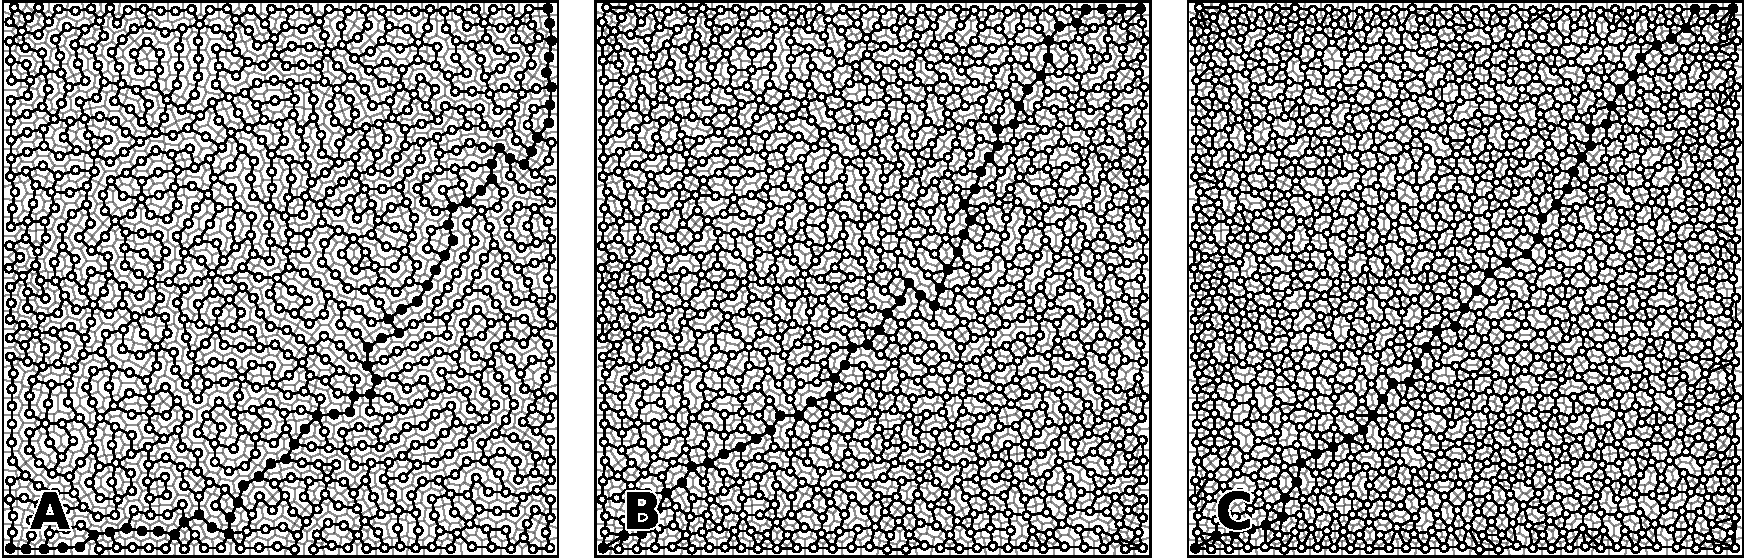
\includegraphics[width=\columnwidth]{figures/distances.pdf}
%\caption{\textbf{Influence of the number of neighbours on the graph distance.} The same initial set of 1003 neurons has been equipped with 2-nearest neighbors, 3 nearest neighbors and 4-nearest neighbors induced topology (panels \textbf{A}, \textbf{B} and \textbf{C} respectively). A sample path from the the lower-left neuron to the upper-right neuron has been highlighted with a thick line (with respective lengths of 59, 50 and 46 nodes).}
%  \label{fig:topology}
%\end{figure}


\subsection{Learning}

The learning process is an iterative process between time $t=0$ and time $t=t_f \in \mathbb{N}^+$ where vectors $\mathbf{v} \in \Omega$ are sequentially presented to the map. For each presented vector $\mathbf{v}$ at time $t$, a winner $s \in \mathcal{N}$ is determined according to equation (\ref{eq:psi}). All codes $\mathbf{w}_{i}$ from the code book are shifted towards $\mathbf{v}$ according to
\begin{equation}
  \Delta\mathbf{w}_{i} = \varepsilon(t)~h_\sigma(t,i,s)~(\mathbf{v} -
  \mathbf{w}_i)
  \label{eq:som-learning}
\end{equation}
with $h_\sigma(t,i,j)$ being a neighborhood function of the form
\begin{equation}
  h_\sigma(t,i,j) = e^{- \frac{{d^p_{ij}}^2}{\sigma(t)^2}}
  \label{eq:som-neighborhood}
\end{equation}
where $\varepsilon(t) \in \mathbb{R}$ is the learning rate and $\sigma(t) \in \mathbb{R}$
is the width of the neighborhood defined as
\begin{equation}
  \sigma(t) =
  \sigma_i\left(\frac{\sigma_f}{\sigma_i}\right)^{t/t_f}, \text{ with } \varepsilon(t) =
  \varepsilon_i\left(\frac{\varepsilon_f}{\varepsilon_i}\right)^{t/t_f},
\end{equation}
while $\sigma_i$ and $\sigma_f$ are respectively the initial and final neighborhood width and $\varepsilon_i$ and $\varepsilon_f$ are respectively the initial and final learning rate. We usually have $\sigma_f \ll \sigma_i$ and $\varepsilon_f \ll \varepsilon_i$.

%The learning algorithm we propose in this work relies on the standard SOM algorithm~\cite{Kohonen:1982}. Once we have define the topology of the map following the steps we described in paragraph~\ref{sec:topo}, we can start the learning process. Learning is iterative and starts at a time $t_0=0$ and runs until some predetermined final time step, $t_f \in \mathbb{N}^+$, has been reached. At every iteration input vectors $\mathbf{v} \in \Omega$ are sequentially given to the map with respect to the probability density function $f$ \gid{Where is defined?}. For each vector $\mathbf{v}$ at time $t$, a winner neuron with index  $s \in \mathcal{N}$ is determined according to equation (\ref{eq:psi}). This means that at time $t$ neuron $s$ is closer to the input vector ${\bf v}$, in the sense of Euclidean distance, than any other neuron. Once the winner neuron has been identified all codes $\mathbf{w}_{i}$ from the current code book are shifted towards $\mathbf{v}$ according to
%\begin{align}
%\label{eq:som-learning}
%    \Delta\mathbf{w}_{i} &= \varepsilon(t)~h(t,i,s;\sigma)~(\mathbf{v} - \mathbf{w}_i), 
%\end{align}
%where $s$ is the index of the winner neuron, $i$ is the index of code words in the code book and $t$ is the current time step. $h_\sigma(t,i,j;\sigma)$ is a neighborhood function of the form
%\begin{equation}
%  h(t,i,j; \sigma) = \exp\Big(-\frac{{d_{ij}}^2}{\sigma(t)^2}\Big)
%  \label{eq:som-neighborhood}
%\end{equation}
%where $\varepsilon: \mathbb{R} \rightarrow \mathbb{R}$ is the learning rate time-dependent function given by $\varepsilon(t) = \varepsilon_i\left(\frac{\varepsilon_f}{\varepsilon_i}\right)^{t/t_f}$, where $\varepsilon_i$ and $\varepsilon_f$ are the initial and final learning rates, respectively. $\sigma: \mathbb{R} \rightarrow \mathbb{R}$ is determines the width of the  neighborhood function~\eqref{eq:som-neighborhood} and it is reads $\sigma(t) = \sigma_i\left(\frac{\sigma_f}{\sigma_i}\right)^{t/t_f}$, where $\sigma_i$ and $\sigma_f$ are the initial and final neighborhood widths, respectively. We usually assume $\sigma_f \ll \sigma_i$ and  $\varepsilon_f \ll \varepsilon_i$. The entire learning procedure is summarized by Algorithm~\ref{algo:vsom}. 

%% %%
\begin{algorithm}[!htpb]
	\begin{algorithmic}
    	\Require $\mathcal{S}$, $\mathcal{N}$, $t_f$, $dt$, $\varepsilon_i$, $\varepsilon_f$, $\sigma_i$, $\sigma_f$
        \Ensure ${\bf W}$
        \If {\text{Blue noise is True}}
        	\State Compute blue noise distribution $\mathcal{B}$
        	\State Compute $e_{ij} = || p_i - p_j ||$		\Comment{Euclidean pair distances matrix}
        	\State Construct matrix ${\bf G}_m$			\Comment{Connectivity matrix}
        	\State Compute matrix ${\bf D}_m$			\Comment{Shortest paths between nodes}
        	\State Place neurons positions on points sampled from $\mathcal{B}$
        \Else
        	\State Discretize grid $[0, 1]\times[0, 1]$ and place neurons on its nodes
        \EndIf
        
        \State $w_s \gets \varnothing$, ${\bf W} \sim \mathcal{U}(0, 1)$	\Comment{Initialize winner unit and code book}
                 
        \For{$t \gets 0, \ldots, t_f$}
        	\State ${\bf v} \gets \bf{s}_t $	\Comment{${\bf s}_t \in \mathcal{S}$}
        	\State $s \gets argmin_{i \in \mathcal{N}} (\lVert \mathbf{v} - \mathbf{w}_i \rVert)$
        	\State $\varepsilon(t) = \varepsilon_i\left(\frac{\varepsilon_f}{\varepsilon_i}\right)^{t/t_f}$
        	\State $\sigma(t) = \sigma_i\left(\frac{\sigma_f}{\sigma_i}\right)^{t/t_f}$
        	\State $h(t,i,j; \sigma) = \exp\Big(-\frac{{d_{ij}}^2}{\sigma(t)^2}\Big)$
        	\State ${\bf w}_i^{\text{new}} = {\bf w}_i^{\text{old}} + \varepsilon(t) \odot h(t,i,s;\sigma) \odot (\mathbf{v} - \mathbf{w}_i^{\text{old}})$
        \EndFor
	\end{algorithmic}
\caption{Voronoi Self-organizing Map (vSOM). $\mathcal{N}$ is neurons index set,
$\mathcal{I}$ is the input dataset, $t_f$ is the simulation time (or the number of input samples).
$\varepsilon_i$ and $\varepsilon_f$ are the initial and final learning rates,
respectively. $\sigma_i$ and $\sigma_f$ are the initial and final neighborhood
widths. $\odot$ is the Hadamard product.}
\label{algo:vsom}
\end{algorithm}
%%


\subsection{Analysis Tools}
In order to analyze and compare the results of RSOM and SOM, we used a spectral method and persistence diagram analysis on the respective codebooks. These analysis tools are detailed below but roughly, the spectral method allows to estimate the distributions of eigenvalues in the activity of the maps while the persistence diagram allows to check for discrepancies between the topology of the input space and the topology of the map.

% To analyze the results of both the Kohonen SOM and VSOM algorithms and to make any comparison between the two algorithms we use a spectral method and persistence diagram on codebooks. The spectral method estimates the distributions of eigenvalues of the activity of neurons. The persistence diagram is a topological-geometrical  approach, more precisely is a tool coming from the field of topological data analysis (TDA). TDA provides the tools to investigate the topology of the maps and the input space and spot differences between the topology of the input space and the neural space of the SOM algorithms (Kohonen and VSOM). 

%\subsubsection{Topological Data Analysis}
\label{sec:tda}

Topological Data Analysis (TDA) \citep{Carlsson:2009} provides methods and tools to study topological structures of data sets such as point cloud and is useful when geometrical or topological information is not apparent within a data set. Furthermore, TDA tools are insensitive to dimension reduction and noise which make them well suited to analyze high-dimensional self-organized maps and their corresponding input data sets. In this work, we use the notion of persistent barcodes and diagrams \citep{Edelsbrunner:2008} to spot any differences between the topology of the input and neural spaces. Furthermore, we can apply some metrics from TDA such as the Bottleneck distance and measure how close two persistent diagrams are.

\correction { We provide, here, a simple example of how we used TDA to
  extract information relative to the underlying topology of input and
  neural spaces (a more rigorous description of the methods used in this work
  are given in section~\ref{sec:si_tda} of SI).
  Figure~\ref{fig:tda_example} illustrates a complete example of how we apply
  TDA in this work. First we need to collect the data (point cloud). In our
  example the data are either the $2$-dimensional points of the input space or
  the codebooks of the neural space (see panel A of
  Figure~\ref{fig:tda_example}). Once we have the point cloud we apply
  a filtration process, where a disc of a specific radius, $\alpha$ is
  drawn around each point. We increase the radius systematically and
  all the intersected discs are registered. In
  figure~\ref{fig:tda_example} B, radius $\alpha_1$ is too small and
  therefore there are no intersected discs. The simplicial complex
  (see section~\ref{sec:si_tda} for more details) in this case is a
  set of points (\emph{i.e.}, simplex $0$). The isolated points in the 
  bottom panel of figure~\ref{fig:tda_example}B define the homology group
  $H0$. This can be seen also in the persistence barcode shown in
  figure~\ref{fig:tda_example}E, where the blue lines correspond to the
  isolated points. The beginning of the line segment indicates the
  radius at which each point is born and the end of the line shows when it
  vanished (died). A line segment on the persistent barcode
  (figure~\ref{fig:tda_example}F) or a point on the persistent diagram
  (figure~\ref{fig:tda_example}E) appears when a disc is applied on a
  data point (birth) and it is preserved until the disc intersects
  another disc (or other discs). Then the line segment or the point
  dies and a new one that represents the joint (intersected discs)
  appear in the persistent barcode or diagram.  If a point persists
  the most then that point considered significant from a topological
  point of view. }

\correction{Back to our example, the radius $\alpha$ is increased
  until some discs intersect each other ($\alpha_2$, panel C).  When
  two discs intersect, we connect their centers (dots) with a line
  segment (\emph{i.e.}, simplex $1$). In figure~\ref{fig:tda_example}C, bottom
  panel, we see that there is a closed path formed by the connected
  linear segments and there is a hole in the complex.  This hole
  corresponds to an $H1$ homology group and the isolated point (or
  points) to $H0$ homology. The persistent barcode reveals the
  formation of a hole when the radius reaches the $\alpha_2$ and the
  orange linear segment first appears in figure~\ref{fig:tda_example}E. The
  other orange line segment corresponds to some other radius that is not
  shown for illustration purposes. Increasing the radius even
  further, we get larger discs and now in some cases, more than two
  discs intersect. When three discs intersect we obtain a triangle
  (simplex $2$, pink triangles in panel D) and when four discs
  intersect we get a tetrahedron (simplex $3$, blue color in panel D), etc.
  Both the triangles and the tetrahedron are not important topological
  features and thus we ignore them. What is important here is the
  number of isolated points, holes an voids (we are not considering
  voids in this example). }

\correction{By following the procedure described in the
  aforementioned example, for any $n$-dimensional inputs, we can
  obtain the persistence barcodes and diagrams, like the ones in
  figures~\ref{fig:tda_example} \textbf{E} and \textbf{F},
  respectively. By inspecting the barcodes we can decide if there is
  any important (persistent) topological feature. Furthermore, we can
  compare quantitatively the persistence diagrams by using distance
  functions such as the Bottleneck distance~\citep{Chazal:2017}. Thus
  we can examine how close two persistence diagrams are and hence, we
  can infer how the self-organizing maps retain or degenerate the
  topology of the input space since we compare the persistence of
  input space against the codebooks of the neural space. Therefore, we
  can compare the input space against the learned codebooks of our
  algorithm (RSOM) and those learned by Kohonen's SOM. Finally, we can
  draw some conclusions on which algorithm retains the topology of
  input space the best. For the analysis in this work we used the
  Gudhi library~\citep{Maria:2014}. In section~\ref{sec:si_tda}, we
  provide a rigorous description of how we compute the persistent
  barcodes and diagrams and we give more details on the tools we
  used. }


\begin{figure}[!htpb]
    \centering
    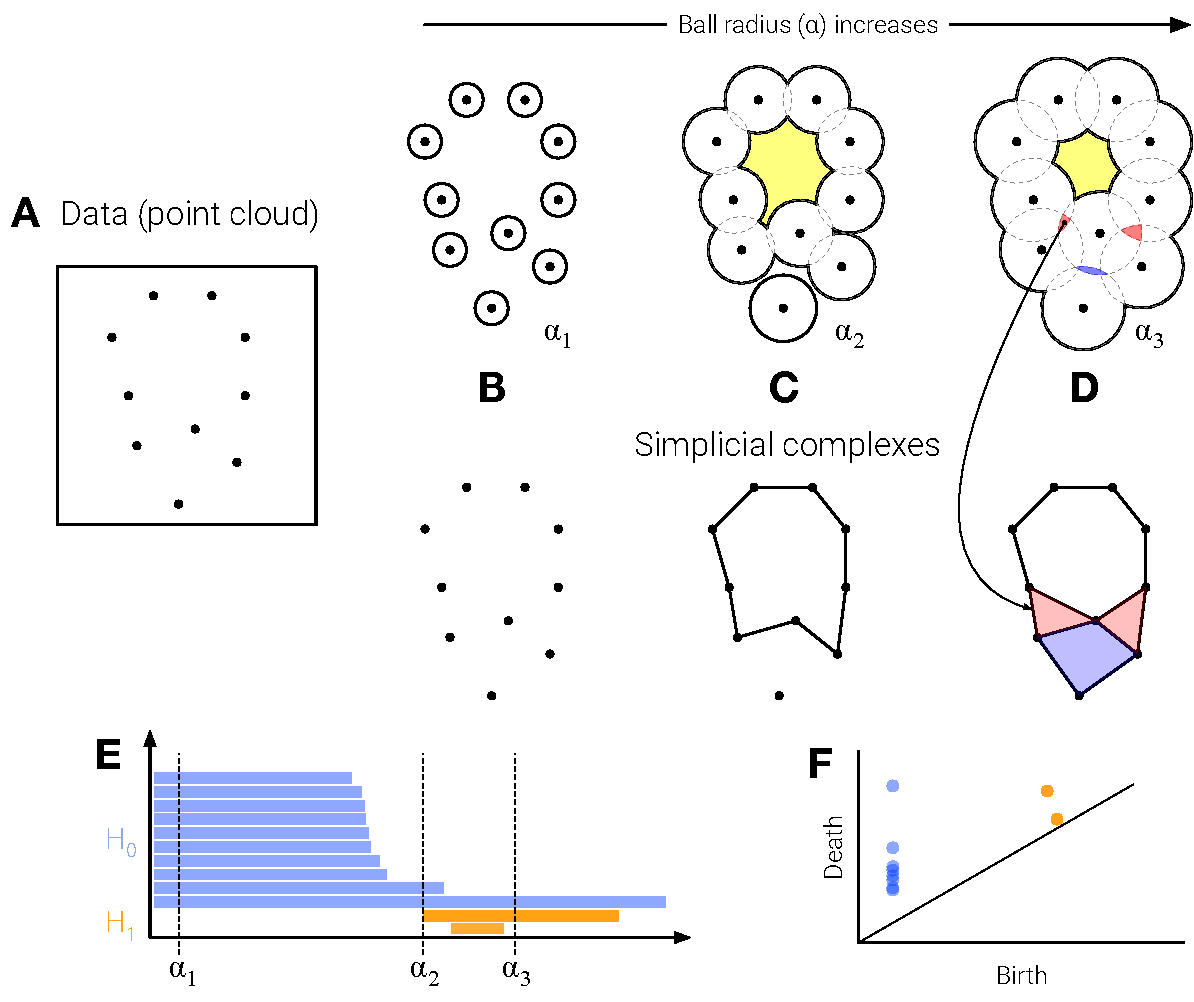
\includegraphics[width=0.8\textwidth]{TDA.pdf}
    \caption{\textbf{Example of Topological Data Analysis.}
      \textbf{A} Point cloud (input data to TDA algorithm). In our
      case this can be either the data points of the input space or
      the codebooks of neural space. The filtration begins with discs
      of small radius $\alpha$ placed on the data points. For
      instance, in \textbf{B} we have small discs (radius is
      $\alpha_1$) and we observe that no disc intersect with
      another. Therefore the simplicial complex in this case is just a
      set of points (bottom panel of \textbf{B}). Then the radius is
      being increased to $alpha_2$ and we see in \textbf{C} that now
      many intersecting discs appear. Whenever two discs intersect we
      connect their centers with a line segment and we obtain the
      simplicial complex at the bottom panel. In this case we have a
      circle (hole marked in orange color) and a disconnected point.
      This hole is reflected in the persistent barcode (see panel E)
      as the longer orange line segment (H1 homology).  In \textbf{D}
      the radius is being further increased to $\alpha_3$ and thus
      more discs are now intersecting with each other. In this case
      there are three or four discs intersecting and thus triangles
      (simplex $3$) and tetrahedrons are formed (see the purple and
      pink colors in the bottom panel, respectively). However, the
      hole that formed when the radius was set to $\alpha_2$ is still
      present (persists) and this is reflected to the persistent
      barcode (panel E) by the longer orange line segment.  The
      persistent barcode in \textbf{E} illustrates the isolated points
      and the holes detected during the filtration process. The points
      are represented by the blue line segments and the holes by the
      orange ones. We call the former $H0$ group (homology $0$) and
      the latter $H1$ homology. A similar representation is given by
      the persistence diagram in \textbf{F}, where each dot represents
      a pair of (birth, death) of a persistent feature. For instance,
      when we apply the discs on data points for first time we mark
      the birth and once the discs intersect for first time then the
      two points that correspond to the intersected discs die and one
      new is generated (the two center of discs have been joined with
      a line segment). In the persistent diagram the blue dots
      correspond to $H0$ and orange ones to $H1$ homology.}
    \label{fig:tda_example}
\end{figure}




\subsection{Simulation Details}

Unless specified otherwise, all the models were parameterized using values given in table \ref{table:parameters}. These values were chosen to be simple and do not really impact the performance of the model. All simulations and figures were produced using the Python scientific stack, namely, SciPy \citep{Jones:2001}, Matplotlib \citep{Hunter:2007}, NumPy \citep{Walt:2011}, Scikit-Learn \citep{Pedregosa:2011}. Analysis were performed using Gudhi \citep{Maria:2014}). 
Sources are available at \href{https://github.com/rougier/VSOM}{github.com/rougier/VSOM}.
%%
\begin{table}[!ht]
  \begin{center}
    \begin{tabular}{ll}
        \textbf{Parameter} & \textbf{Value} \\
        \hline
        Number of epochs      ($t_f$)           & 25000\\
        Learning rate initial ($\varepsilon_i$) & 0.50\\
        Learning rate final   ($\varepsilon_f$) & 0.01\\
        Sigma initial         ($\sigma_i$)      & 0.50\\
        Sigma final           ($\sigma_f$)      & 0.01\\
    \end{tabular}
      \caption{\textbf{Default parameters} Unless specified otherwise, these are
        the parameters used in all the simulations.}
      \label{table:parameters}
  \end{center}
\end{table}

%We conduct all the experiments using the parameters provided by Table~\ref{table:parameters}. In all the experiments the input space is the Cartesian product $[0, 1] \times [0, 1]$ and neurons positions drawn from a blue noise distribution using the fast Poisson disk sampling algorithm~\cite{Bridson:2007} (see paragraph~\ref{sec:spatial_dist} for more details).  The source code of the proposed algorithm is written in the Python programming language (SciPy~\cite{Jones:2001}, Matplotlib~\cite{Hunter:2007} and NumPy~\cite{Walt:2011}, Scikit-Learn~\cite{Pedregosa:2011}, Gudhi~\cite{Maria:2014}). Sources are available at \href{https://github.com/rougier/VSOM}{github.com/rougier/VSOM}.


%% Considering a set of $n$ points $P = \{P_i\}_{i \in [1,n]}$ on a finite domain
%% $D \in \mathbb{R}^2$, the Voronoi tesselation $V(P) = \{V_i\}_{i \in [1,n]}$ of
%% $P$ is defined as:
%% %
%% \begin{equation}
%%   \forall i \in [1,n], V_i = \{x \in D \mid
%%   \lVert x - P_i \rVert \leq \lVert x - P_j \rVert, \forall j \neq i\}
%% \end{equation}
%% %
%% Reciprocally, the (unique) Delaunay triangulation $T(P) = \{T_i\}_{i \in
%%   [1,n]}$ of $P$ is the dual graph of the Voronoi diagram and defined such that
%% no point in $P$ is inside the circumcircle of any triangles in $T(P)$. The
%% centers of the circumcircles are equivalent to the Voronoi diagram, i.e. a
%% partition of $D$ into Voronoi cells. For each of the cell $V_i$, we can compute
%% its centroid $C_i$ which is the center of mass of the cell. A Voronoi
%% tesselation is said to be centroidal when we have $\forall i \in [1,n], C_i =
%% P_i$ (see figure~\ref{fig:CVT}).\\

%% For an arbitrary set of points, there is no guarantee that the corresponding
%% Voronoi tesselation is centroidal but different methods can be used to
%% generate a centroidal tesselation from an arbitrary set of points. One of the
%% most straightforward and iterative methods is the Lloyd relaxation scheme
%% \cite{Lloyd:1982}:
%% \begin{enumerate}
%%   \item The Voronoi diagram of the $n$ points is computed
%%   \item The centroid of each of the $n$ Voronoi cell is computed.
%%   \item Each point is moved to the corresponding centroid of its Voronoi cell
%%   \item The method terminates if criterion is met (see below), else go to 1
%% \end{enumerate}
%% The algorithm finishes when the maximum distance between points and centroids
%% is less than a given threshold as illustrated in figure~\ref{fig:CVT}. It is
%% to be noted that because of numerical imprecisions, there is no guarantee that
%% an arbitrary small threshold can be reached.


%% \begin{figure}[htbp]
%%   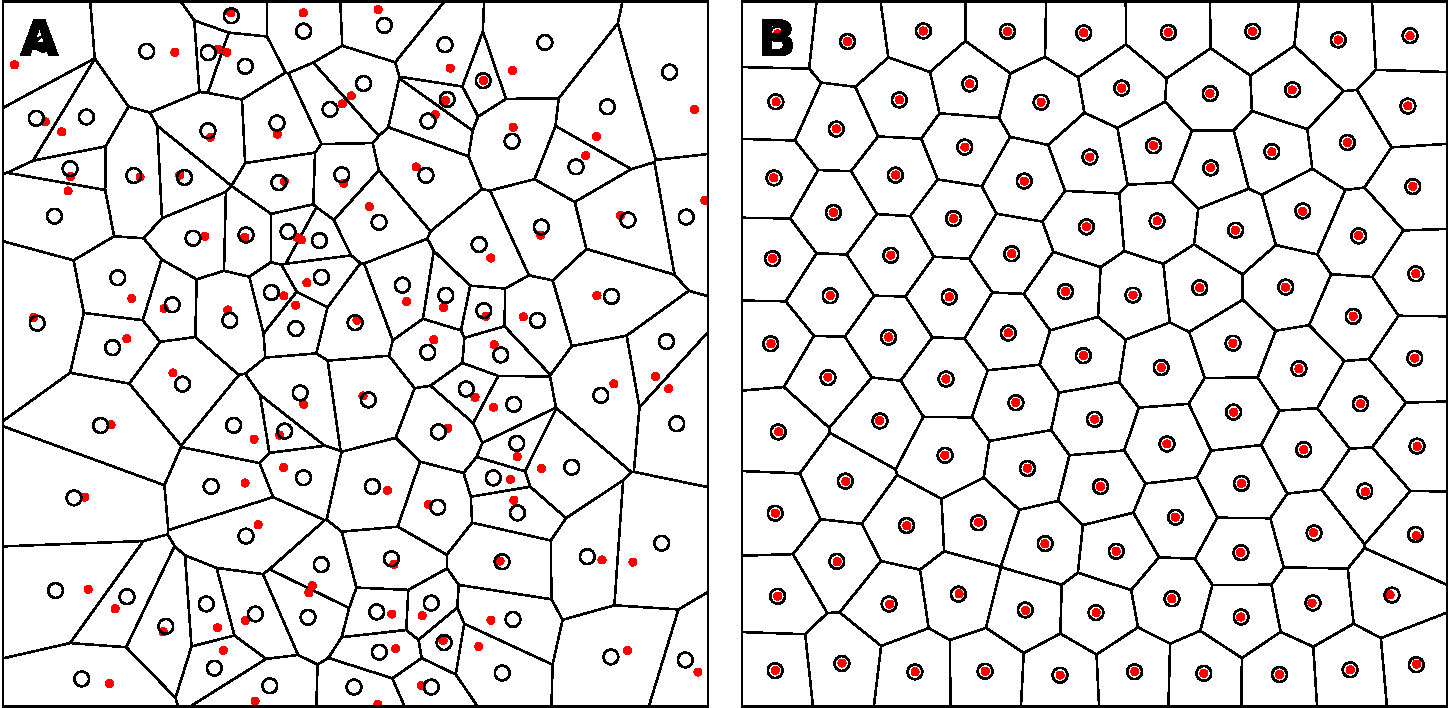
\includegraphics[width=\textwidth]{figures/CVT.pdf}
%%   \caption{\textbf{Centroidal Voronoi Tesselation.}  \textbf{\textsf{A.}}
%%     Voronoi diagram of a uniform distribution (n=100) where red dots represent
%%     the uniform distribution and white circles represent the centroids of each
%%     Voronoi cell. \textbf{\textsf{B.}} Centroidal Voronoi diagram where the
%%     point distribution matches the centroid distribution which constitutes a
%%     blue noise distribution (i.e. {\em a distribution that is roughly uniformly
%%       random with no preferred inter-point directions or distances} according
%%     to the definition of \cite{Ebeida:2014}). This figure has been obtained
%%     from the initial distribution on the left after 50 iterations of the Lloyd
%%     relaxation algorithm. }
%%   \label{fig:CVT}
%% \end{figure}
%
